\chapter{Mining} \label{sec:mining}
%
\epigraph{Security is a binary state. A system cannot be secure against malicious attackers and insecure against other "noble" parties. It is either secure or insecure. And if the prospect of an attack exists, then security collapses.}{\textit{Edward Snowden}}
\section{Introduction}
%%%%%%%%%%%%%%%%%%%%%%%%%%%%%%%%%%%%%%%%%%%%%%%%%%%%%%%%%%%%%%%%%%%%%%%%%%%%%%%%
%% Think about it, seems ugly
\setlength{\intextsep}{0pt}
\begin{wrapfigure}[10]{L}{0.3\textwidth}
\centering
\includegraphics[width=0.30\textwidth]{Images/Bitcoin/mining_start.jpg}
\end{wrapfigure}
%%%%%%%%%%%%%%%%%%%%%%%%%%%%%%%%%%%%%%%%%%%%%%%%%%%%%%%%%%%%%%%%%%%%%%%%%%%%%%%%
Mining\footnote{It is misleading to think that there is an analogy between gold mining and cryptocurrency mining. The fact is that gold miners are rewarded for producing gold, while some cryptocurrency's miners are not rewarded for producing cryptocoins; they are rewarded for their record-keeping services.} is the processing of transactions in the digital currency system, in which the records of some cryptocurrency's current  transactions, \hyperref[sec:blocks]{\emph{blocks}} (see \hyperref[sec:blocks]{section}~\ref{sec:blocks}), are added to the record of past transactions, the \hyperref[sec:blockchain]{\emph{blockchain}} (see \hyperref[sec:blockchain]{section}~\ref{sec:blockchain}). Miners keep the blockchain consistent, complete, and unalterable by repeatedly grouping newly broadcast transactions into a block, which is then broadcast to the network and verified by recipient nodes~\cite{economist}. Each block contains a SHA-256 cryptographic hash of the previous block~\cite{economist}, thus linking it to the previous block and giving the blockchain its name.

To be accepted by the rest of the network, a new block must contain a \hyperref[sec:proofofwork]{Proof of Work (PoW)} (see \hyperref[sec:proofofwork]{section}~\ref{sec:proofofwork}). The PoW requires miners to find a number called a nonce, such that when the block content is hashed along with the nonce, the result is numerically smaller than the network's difficulty target~\cite{Nakamoto_bitcoin:a} and thus the \hyperref[eq:PoW]{PoW equation} (see \hyperref[eq:PoW]{equation}~\ref{eq:PoW}) is satisfied. This proof is easy for any node in the network to verify, but extremely time-consuming to generate, as for a secure cryptographic hash, miners must try many different nonce values before meeting the difficulty target.

The primary purpose of mining is to set the history of transactions in a way that is computationally impractical to modify by any one entity. By downloading and verifying the blockchain, nodes are able to reach consensus about the ordering of events in some proof of work cryptocurrency~\cite{wiki}.

As we noted in \hyperref[sec:proofofwork]{section}~\ref{sec:proofofwork}, every 2,016 blocks the difficulty target is adjusted based on the network's recent performance, with the aim of keeping the average time between new blocks at ten minutes. In this way, the system automatically adapts to the total amount of mining power on the network. Between 1 March 2014 and 1 March 2015, the average number of nonces, miners had to try before creating a new block, increased from 16.4 quintillion to 200.5 quintillion~\cite{difficulty_history}.

The proof of work system, alongside the chaining of blocks, makes modifications of the blockchain extremely hard, as an attacker must modify all subsequent blocks in order for the modifications of one block to be accepted. As new blocks are mined all the time, the difficulty of modifying a block increases as time passes and the number of subsequent blocks (also called confirmations of the given block) increases~\cite{economist}.

Mining is also the mechanism used to introduce coins into the system: Miners are paid any transaction fees as well as a "subsidy" of newly created cryptocoins. This both serves the purpose of disseminating new cryptocoins in a decentralized manner as well as motivating people to provide security for the system~\cite{wiki}. To elaborate on the second part of this purpose, one can think about the structure of the consensus on the network. The network agrees by majority. So an attacker who controls 51\% of the mining power can successfully attack this structure. As more honest miners contribute to the network, the 51\% attack becomes less feasible.

\begin{wrapfigure}{R}{0.52\textwidth}
  \centering
  \includegraphics[width=0.52\textwidth,keepaspectratio]{Images/Bitcoin/mining.jpeg}
  \caption{Mining options}
  \label{fig:mining}
\end{wrapfigure}
Originally, Bitcoin mining was conducted on the CPUs of individual computers, with more cores and greater speed resulting in more profitability. After that, the system became dominated by multi-graphics card systems, then field-programmable gate arrays (FPGAs) and finally application-specific integrated circuits (ASICs), in the attempt to find more hashes per hour with less electrical power usage (see \hyperref[fig:mining]{figure}~\ref{fig:mining}).

Due to this constant escalation, it has become hard for prospective new miners to start. This adjustable difficulty is an intentional mechanism created to prevent inflation. To get around that problem, individuals often work in \emph{mining pools}. Mining pools are groups of miners who join their collective computational power and share their profit according to the contribution of each party.

Bitcoin generally started with individuals and small organizations handling the mining. At that time, start-up could be enabled by a single high-end gaming system. However, nowadays larger mining organizations might spend tens of thousands on one high-performance, specialized, application-specific integrated circuit.

That creates a problem. In a system, which since its creation is supposed to distribute power among users, there has been a great power concentration in the hands of big companies, like Bitfury or 21, that develop ASICs to mine Bitcoin. Because of the extreme cost of ASICs and extreme hashrate, someone who uses a multi-graphics card system or a CPU is out of competition. As a result, independent miners have largely dried up.

\section{Egalitarian Mining} \label{sec:egalitarian}
\setlength{\intextsep}{0pt}
\begin{wrapfigure}[7]{L}{0.32\textwidth}
\centering
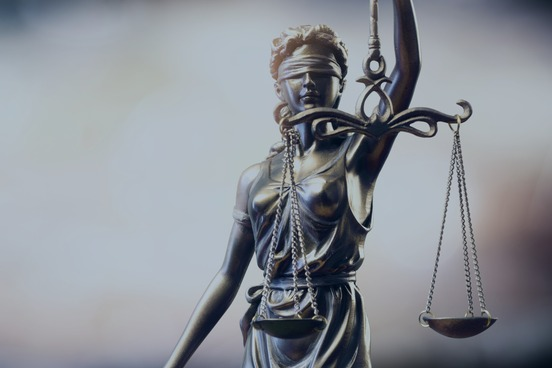
\includegraphics[width=0.32\textwidth]{Images/Mining/justice.jpg}
\end{wrapfigure}
Let's consider several contexts where an adversary has an upper hand over the defender, by using special hardware in an attack. These include password processing, hard-drive protection, cryptocurrency mining, resourse sharing, code obfuscation, etc. \hyperref[sec:memory-hard]{Memory-hard} computing is a generic paradigm, which can protect the defender against attacks in the aforementioned contexts. Every task is amalgamated with a certain procedure requiring intensive access to RAM, both in terms of size and bandwidth, so that transferring the computation to GPU, FPGA, and even ASIC brings little to no cost reduction.

Cryptographic schemes that run in this framework become \emph{egalitarian} in the sense that both users and attackers are equal in the price-performance ratio conditions. When the cryptographic scheme is a hash function used for cryptocurrency mining, we refer to this notion as \emph{egalitarian mining}.

But let's step back a little and think about the need for such a notion. Do we actually need it? Is egalitarian mining a way to destroy competition? Is it unfair? Shouldn't a miner be rewarded for the extra money he invested?

Many questions like the above have been asked and usually the answer is not descriptive enough of what really memory-hardness introduces to the world. We will try here to demonstrate concretely what it means for a cryptocurrency to offer egalitarian mining.

\emph{Egalitarian mining does not destroy competition.} The miner who invests more in hardware is rewarded more. Each individual miner is rewarded according to the computation power he offers to the community. The real difference is that it is really easy for people to start mining with a single high-end gaming system. Hobbyists, who want to support the community are welcome to mine. In Bitcoin system, this option is not available. In order to support the community by mining, you have to invest a lot of money on ASICs to be competitive. This means that, in general, the mining to support the Bitcoin project or for fun is dead.

This is hurtful for a system, which by design is supposed to bring decentralization in the financial market. Because, without hobbyists, we are actually left with big companies handling almost all of the mining. Companies will comply with regulations that the government of each country enforces and cannot be expected to react and inspire political movements. Since countries can and they have, historically, collaborated against threats, a union of countries who can enforce regulations to companies that control more than 51\% of the hashing power, can bring a cryptocurrency to its knees, if seen as a threat. That scenario does not fit in most definitions of security.

One of the reasons that cryptocurrencies have a bootstrapping period is because they need a big support community to distribute mining in order to guarantee security. When the total hashing power is a few high-end gaming systems, acquiring 51\% of the hashing power is feasible. As the support expands, the security is satisfied for all practical purposes. But when mining is dominated by companies, then a totally trustless system gives birth to a trusted party. That's against the motivation for the inception of a cryptocurrency and it raises questions like "\emph{Why should I trust the mining companies and support this cryptocoin? Do I trust my bank more? After all, my bank is just another company...}"
\pagebreak

\subsection{Formal definition}
Now the reader should have a good understanding about the notion of \emph{egalitarianism}. However, the claims for egalitarianism in several cryptocurrencies have been hand wavy and no such claim is accompanied by exact data. Egalitarianism was a vague and undefined term until quite recently. In 2019, Dimitris Karakostas, Aggelos Kiayias, Christos Nasikas and Dionysis Zindros published a paper~\cite{egalitarianism} aiming to end this era of ambiguity. They presented a quantitative definition for this term and set the basis for future work in this direction.

As a means towards establishing their definition, they define the \emph{egalitarian curve} $f$ of a cryptocurrency. Reproduced from~\cite{egalitarianism}:
\begin{fverbatim}{?}
  The horizontal axis of this curve plots the financial capital
  which is available for investment denominated in a fiat
  currency?Fiat currency is legal tender whose value is backed by the government that issued it. The U.S. dollar is fiat money, as are the euro and many other major world currencies. A fiat currency's value is underpinned by the strength of the government that issues it, not its worth in gold or silver. ?, USD. The vertical axis plots the Return On
  Investment (ROI), which measures the cryptocurrency amount that
  is freshly generated in the investment period and remains
  unspent at the end of the investment period, given an optimal
  allocation of the initial capital.
\end{fverbatim}

They continue with the necessary definition of the \emph{egalitarian curve} in order to prepare a concrete and sound definition of the term \emph{egalitarianism}. We reproduce here the two definitions. Again, from the \cite{egalitarianism}:

\begin{definition}[Egalitarian curve]
    Given a cryptocurrency $c$, an investment period interval $d$, the set of
    all possible investment strategies $\mathcal{B}$, we define the \emph{egalitarian curve}
    $f_{c,d}: \mathbb{R}^+ \longrightarrow \mathbb{R}^+$ of $c$ for
    investment period $d$ as:

    \begin{equation} \nonumber
      f_{c,d}(v) = \frac{\underset{B \in \mathcal{B}}{\max}{\mathbb{E}[B(v)]} - v}{v}
    \end{equation}
\end{definition}

The value $\underset{B \in \mathcal{B}}{\max}{\mathbb{E}[B(v)]}$ identifies the maximum expectation of
returns across all investment strategies $\mathcal{B}$, i.e., the amount of
returns which the \emph{optimal} strategy ensures for a given initial capital $v$. Now, we are ready to reproduce their definition of the notion of interest:

\begin{definition}[Egalitarianism]
  Given a cryptocurrency $c$, an investment period duration $d$ and an initial
  capital distribution $\mathcal{D}$, we define the \emph{egalitarianism} $e$ of $c$
  for investment duration $d$ under initial capital distribution $\mathcal{D}$
  as follows:

  \begin{equation} \nonumber
    e_{c,d,\mathcal{D}} = -\textsf{Var}_{v \gets \mathcal{D}}[f_{c,d}(v)]
  \end{equation}
  where $f$ is the egalitarian curve of $c$.
\end{definition}

As they remark in their paper, the intuition behind this definition is that, to have egalitarianism, the ROI must remain the same across different capital investments. As such, any deviation from the mean is non-egalitarian. For further reading the reader is refered to their work~\cite{egalitarianism}.
\pagebreak

We are focusing on mining, but one should think about the possibilities of a \hyperref[sec:proofofwork]{Proof of Work (PoW)} (see \hyperref[sec:proofofwork]{section}~\ref{sec:proofofwork}) mechanism in order to understand the contribution of a memory-hard hash function. The PoW mechanism is actually a voting system. Users vote for the right order of the transactions, for enabling new features in the protocol and for the honest money supply distribution. Therefore, it is important that during the voting process all participants have equal voting rights.

To sum up, for security and decentralization arguments, it is healthy for some cryptocurrency's mining power to be distributed among users. Memory-hardness sustains the competition, but it makes it less harsh and keeps the door open for hobbyists to support the community. It is extremely difficult for the corporate mining to acquire tremendous power for two reasons and that is essential in a trustless system that aims to remain trustless. The reasons are:
\begin{enumerate}[label=(\greek*)]
  \item It is not that lucrative for companies. If someone makes a big investment, he will get big rewards but not insanely huge rewards leaving every hobbyist out of the mining community.
  \item Even if a lot of companies decide to participate, it is difficult for them to acquire a combined 51\% of the total hashing power (It is no more about what devices you buy, just how many).
\end{enumerate}

Memory-hardness defends a system against the aforementioned prospect and thus strengthens the notion of any PoW cryptocurrency's security.
